\chapter{Quantifying research questions}
\label{ch:quantifyingresearch}

Recall, once again, that at the end of Chapter \ref{ch:corpuslinguistics}, we defined corpus linguistics as 

\begin{quotation}
the investigation of linguistic research questions that have been framed in terms of the conditional distribution of linguistic phenomena in a linguistic corpus.
\end{quotation}

We discussed the fact that this definition covers cases of hypotheses phrased in absolute terms, i.e. cases where the distribution of a phenomenon across different conditions is a matter of all or nothing (as in ``All speakers of American English refer to the front window of a car as \textit{windshield}, all speakers of British English as \textit{windscreen}'') as well as cases where the distribution is a matter of more-or-less (as in ``British English speakers prefer the word \textit{railway} over \textit{railroad} when referring to train tracks, American English speakers prefer \textit{railroad} over \textit{railway}'' or ``More British speakers refer to networks of train tracks as \textit{railway} instead of \textit{railroad} and more American English refer to them as \textit{railroad} instead of \textit{railway}'').

In the case of hypotheses stated in terms of more-or-less, predictions must be stated in quantitative terms which in turn means that our data have to be quantified in some way so that we can compare them to our predictions. In this chapter, we will discuss in more detail how this is done when dealing with different types of data.

%[NOTE TO SELF:] Given that, as mentioned in Chapter \ref{ch:scientificmethod}, Section \ref{sec:scientifichypothesis}, hypotheses stated in relative terms are actually more typical in corpus linguistics than hypotheses stated in absolute terms, one might expect quantitative methods to be at the core of corpus-linguistic research practice. However, this is not the case. Many early corpus-linguistic studies chose to forgo quantification completely, or to treat it impressionistically (stating that one thing seemed to be more common in a given corpus or under a given condition than another). This has changed over the last twenty years, and even though the quantitatively apathetic and/or impressionistic schools of corpus linguistics are no longer dominant, they are still strong. In order to distinguish the more principled quantitative approach taken here from this impressionistic approach, it is now often referred to as \textit{Quantitative Corpus Linguistics} (a distinction first suggested in \citep{stefanowitsch_covarying_2005}, although the term is older).

Specifically, we will discuss three types of data (or ``levels of measurement'') that we might encounter in the process of quantifying the (annotated) results of a corpus query (Section \ref{sec:typesofdata}): nominal data (discussed in more detail in Section \ref{sec:descriptivenominal}), ordinal (or rank) data (discussed in more detail in Section \ref{sec:descriptiveordinal}, and cardinal data (discussed in more detail in Section \ref{sec:descriptivecardinal}. These discussions, summarized in Section \ref{sec:datatypessummary}, will lay the ground work for the introduction to statistical hypothesis testing presented in the next chapter.

\section{Types of data}
\label{sec:typesofdata}

In order to illustrate these types of data, let us turn to a linguistic phenomenon that is more complex than the distribution of words across varieties, and closer to the kind of phenomenon actually of interest to corpus linguists: that of the two English ``possessive'' constructions introduced in Section \ref{sec:reliabilityannotationschemes} in Chapter \ref{ch:retrievalannotation} above. As discussed there, the two constructions can often be used seemingly interchangeably, as in (\ref{ex:sgenvsof}a, b):

\begin{exe}
\ex
\begin{xlist} 
\label{ex:sgenvsof}
\ex \textit{The city's museums} are treasure houses of inspiring objects from all eras and cultures. (www.res.org.uk)
\ex Today one can find the monuments and artifacts from all of these eras in \textit{the museums of the city}. (www.travelhouseuk.co.uk)
\end{xlist}
\end{exe}

However, there are limits to this interchangeability. First, there are a number of relations that are exclusively encoded by the \textit{of}-construction, such as quantities (both generic, as in \textit{a couple/bit/lot of}, and in terms of measures, as in \textit{six miles/years/gallons of}), type relations (\textit{a kind/type/sort/class of}) and composition or constitution (\textit{a mixture of water and whisky}, \textit{a dress of silk}, etc.) \citep[cf. e.g.][]{rohdenburg_constructional_2003}.

Second, and more interestingly, even where a relation \textit{can} be expressed by both constructions, there is often a preference for one or the other in a given context. A number of factors underlying these preferences have been suggested and investigated using quantitative corpus-linguistic methods. Among these, there are three that are widely agreed upon to have an influence, namely the givenness, animacy and weight of the modifier. These three factors nicely illustrate the levels of measurement mentioned above, so we will look at each of them in some detail.

\textit{(a) Givenness}. Following the principle of Functional Sentence Perspective, if the modifier (the phrase marked by \textit{'s} or \textit{of}) refers given information, the \textit{s}-possessive will be preferred, if the modifier is new, the construction with \textit{of} will be preferred \citep{standwell_genitive_1982}. Thus, (\ref{ex:sgengivenness}a) and (\ref{ex:ofcgivennessb}a) sound more natural than (\ref{ex:sgengivenness}b) and (\ref{ex:ofcgivennessb}b) respectively:

\begin{exe}
\ex
\begin{xlist} 
\label{ex:sgengivenness}
\ex In New York, we visited \textit{the city's} many museums.
\ex[\textsuperscript{??}]{In New York, we visited the many museums \textit{of the city}.}
\end{xlist}
\end{exe}

\begin{exe}
\ex
\begin{xlist} 
\label{ex:ofcgivennessb}
\ex The Guggenheim is much larger than the museums of other major cities.
\ex[\textsuperscript{??}]{The Guggenheim is much larger than other \textit{major cities'} museums.}
\end{xlist}
\end{exe}

\textit{(b) Animacy}. Since animate referents tend to be more topical than inanimate ones and more topical elements tend to precede less topical ones, if the modifier is animate, the \textit{s}-possessive will be preferred, if it is inanimate, the construction with \textit{of} will be preferred (\citealt[cf.][192-203]{quirk_grammar_1972}, \citealt{deane_english_1987}):

\begin{exe}
\ex
\begin{xlist} 
\label{ex:sgenanimacy}
\ex Solomon R. Guggenheim's collection contains some fine paintings.
\ex[\textsuperscript{??}]{The collection of Solomon R. Guggenheim contains some fine paintings.}
\end{xlist}
\end{exe}

\begin{exe}
\ex
\begin{xlist} 
\label{ex:ofcanimacy}
\ex The collection of the Guggenheim museum contains some fine paintings.
\ex[\textsuperscript{??}]{The Guggenheim museum's collection contains some fine paintings.}
\end{xlist}
\end{exe}

\textit{(c) Length}. Since short constituents generally precede long constituents, if the modifier is short, the \textit{s}-possessive will be preferred, if it is long, the construction with \textit{of} will be preferred \citep{altenberg_binominal_1980}:

\begin{exe}
\ex
\begin{xlist} 
\label{ex:sgenlength}
\ex The museum's collection is stunning.
\ex[\textsuperscript{??}]{The collection of the museum is stunning.
}\end{xlist}
\end{exe}

\begin{exe}
\ex
\begin{xlist} 
\label{ex:ofclength}
\ex The collection of the most famous museum in New York is stunning.
\ex[\textsuperscript{??}]{The most famous museum in New York's collection is stunning.}
\end{xlist}
\end{exe}

In all three cases, we are dealing with hypotheses concerning preferences rather than absolute difference. None of the examples with question marks are ungrammatical and all of them could conceivably occur; they just sound a little bit odd. Thus, the predictions we can derive from each hypothesis must be stated and tested in terms of relative rather than absolute differences -- they all involve a predictions stated in terms more-or-less rather than all-or-nothing. Relative quantitative differences are expressed and dealt with in different ways depending on the type of data they involve.

\subsection{Nominal data}
\label{sec:nominaldata}

A nominal variable is a variable whose values are labels for categories that have no intrinsic order with respect to each other (i.e., there is no aspect of their definition that would allow us to put them in a natural order) -- for example, \textvv{Sex}, \textvv{Nationality} or \textvv{Native Language}. If we categorize data in terms of such a nominal variable, the only way to quantify them is to count the number of observations of each category in a given sample and express the result in absolute frequencies (i.e., raw numbers) or relative frequencies (such as percentages). For example, in the population of the world in 2005, there were 92 million native speakers of \textvv{german} and 75 million speakers of \textvv{french}.

We cannot \emph{rank} the values of nominal variables based on intrinsic criteria. For example, we cannot rank the German language higher the French language on the basis of any intrinsic property of German and French. They are simply two different manifestations of the phenomenon \textvv{Language}, part of an unordered set including all human languages.

That we cannot rank them based on intrinsic criteria does not mean that we cannot rank them at all. For example, we could rank them by number of speakers worldwide (in which case, as the numbers cited above show, German ranks above French). We could also rank them by the number of countries in which they are an official language (in which case French, which has official status in 29 countries, ranks above German, with an official status in only 6 countries). But the number of native speakers or the number of countries where a language has an official status is not an intrinsic property of that language -- German would still be German if its number of speakers was reduced by half by an asteroid strike, and French would still be French if it lost its official status in all 29 countries). In other words,
we are not really ranking \textvv{french} and \textvv{german} as values of \textvv{Language} at all; instead, we are ranking values of the variables \textvv{Size of Native Speech Community} and \textvv{Number of Countries with Official Language X} respectively.

We also cannot calculate mean values (``averages'') between the values of nominal variables. We cannot claim, for example, that Javanese is the mean of German and French because the number of Javanese native speakers falls (roughly) halfway between that of German and French native speakers). Again, what we would be calculating a mean of is the values of the variable \textvv{Size of Native Speech Community}, and while it makes a sort of sense to say that the mean of the values \textvv{number of french native speakers} and \textvv{number of german native speakers} was 83.5 in 2005, it does not make sense to refer to this mean as \textvv{number of javanese speakers}. 

%[NOTE TO SELF:] We also cannot claim that English is the mean of German and French because its vocabulary is derived in equal proportions from the Germanic and the Romance language families...

With respect to the three hypotheses concerning the distribution of the \textit{s}-possessive and the \textit{of}-possessive, it is obvious that they all involve at least one nominal variable -- the constructions themselves. These are essentially values of a variable we could call \textvv{Type of Possessive Construction}. We could categorize all grammatical expressions of possession in a corpus in terms of the values \textvv{\textit{s}-possessive} and \textvv{\textit{of}-possessive}, count them and express the result in terms of absolute or relative frequencies. For example, the \textit{s}-possessive occurs \num{22193} times in the BROWN corpus (excluding proper names and instances of the double \textit{s}-possessive), and the \textit{of}-possessive occurs \num{17800} times.\footnote{This is an estimate; it would take too long to go through all \num{36406} occurrences of \textit{of} and identify those that occur in the structure relevant here, so I categorized a random subsample of 500 hits of \textit{of} and generalized the proportion of \textit{of}-possessives vs. other uses of \textit{of} to the total number of hits for \textit{of}).}

As with the example of the variable \textvv{Native Language} above, we can rank the constructions (i.e. the values of the variable \textvv{Type of Possessive Construction} in terms of their frequency (the \textit{s}-possessive is more frequent), but again we are not ranking these values based on an intrinsic criterion, but on an extrinsic one: their corpus frequency in one particular corpus. We can also calculate their mean frequency (\num{19996.5}), but again, this is not a mean of the two constructions, but of their frequencies in one particular corpus.

\subsection{Ordinal data}
\label{sec:ordinaldata}

An ordinal variable is a variable whose values are labels for categories that \emph{do} have an intrinsic order with respect to each other but that cannot be expressed in terms of natural numbers. In other words, ordinal variables are variables that are are defined in such a way that some aspect of their definition allows us to order them without reference to an extrinsic criterion, but that does not give us any information about the distance (or degree of difference) between one category and the next. If we categorize data in terms of such an ordinal variable, we can treat them accordingly (i.e., we can rank them), or we can treat them like nominal data by simply ignoring their inherent order (i.e., we can still count the number of observations for each value and report absolute or relative frequencies. We cannot calculate mean values.

Some typical examples of ordinal variables are demographic variables like \textvv{Education} or (in the appropriate sub-demographic) \textvv{Military Rank}, but also \textvv{School Grades} and the kind of ratings often found in questionnaires (both of which are, however, often treated as though they were cardinal data, see below).

For example, academic degrees are intrinsically ordered: it is part of the definition of a PhD degree that it ranks higher than a master's degree, which in turn ranks higher than a bachelor's degree. Thus, we can easily rank speakers in a sample of university graduates based on the highest degree they have completed. We can also simply count the number of PhDs, MAs, and BAs and ignore the ordering of the degrees. But we cannot calculate a mean: if five speakers in our sample of ten speakers have a PhD and five have a BA, this does not allow us to claim that all of them have an MA degree on average. The first important reason for this is that the size of the difference in terms of skills and knowledge that separates a BA from an MA is not the same as that separating an MA from a PhD: in Europe, one typically studies two years for an MA, but it typically takes four to five years to complete a PhD. The second important reason is that the values of ordinal variables typically differ along more than one dimension: while it is true that a PhD is a higher degree than an MA, which is a higher degree than a BA, the three degrees also differ in terms of specialization (from a relatively broad BA to a very narrow PhD), and the PhD degree differs from the two other degrees qualitatively: a BA and an MA primarily show that one has acquired knowledge and (more or less practical skills), but a PhD primarily shows that one has acquired research skills.

With respect the three hypotheses concerning the distribution of the \textit{s}\hyp{}possessive and the \textit{of}-possessive, clearly \textvv{Animacy} is an ordinal variable, at least if we think of it in terms of a scale, as we did in Chapter \ref{ch:scientificmethod}, Section \ref{sec:operationalization}. Recall that a simple animacy scale might look like this:

\begin{exe}
\ex \textvv{animate} > \textvv{inanimate} > \textvv{abstract}
\label{ex:simpleanimacyscale}
\end{exe}

On this scale, \textvv{animate} ranks higher than \textvv{inanimate} which ranks higher than \textvv{abstract} in terms of the property we are calling ``animacy'', and this ranking is determined by the scale itself, not by any extrinsic criteria.

This means that we could categorize and rank all nouns in a corpus according to their animacy. But again, we cannot calculate a mean. If we have 50 \textvv{human} nouns and 50 \textvv{abstract} nouns, we cannot say that we have 100 nouns with a mean value of \textvv{inanimate}. Again, this is because we have no way of knowing whether, in terms of animacy, the difference between \textvv{animate} and \textvv{inanimate} is the same size as that between \textvv{inanimate} and \textvv{abstract}, but also, because we are, again, dealing with qualitative as well as quantitative differences: the difference between animate and inanimate on the one hand and abstract on the other is that the first two have physical existence; and the difference between animate on the one hand and inanimate and abstract on the other is that animates are potentially alive and the other two are not. In other words, our scale is really a combination of at least two dimensions.

Again, we could ignore the intrinsic order of the values on our \textvv{Animacy} scale and simply treat them as nominal data, i.e., count them and report the frequency with which each value occurs in our data. Potentially ordinal data are actually frequently treated like nominal data in corpus linguistics (cf. Section \ref{sec:mode}, and with complex ``scales'' combining a range of different dimensions, this is probably a good idea; but ordinal data also have a useful place in quantitative corpus linguistics.

\subsection{Cardinal data}
\label{sec:cardinaldata}

Cardinal variables are variables whose values are numerical measurements along a particular dimension. In other words, they are intrinsically ordered (like ordinal data), but not because some aspect of their definition allows us to order them, but because of their nature as numbers. Also, the distance between any two measurements is precisely known and can directly be expressed as a number itself. This means that we can perform any arithmetic operation on cardinal data -- crucially, we can calculate means. Of course, we can also treat cardinal data like rank data by ignoring all of their mathematical properties other than their order, and we can also treat them as nominal data.

Typical cases of cardinal variables are demographic variables like \textvv{Age} or \textvv{Income}. For example, we can categorize a sample of speakers by their age and then calculate the mean age of our sample. If our sample contains 5 50-year-olds and 5 30-year-olds, it makes perfect sense to say that the mean age in our sample is 40; we might need additional information to distinguish between this sample and another sample that consists of 5 41-year-olds and 5 39-year-olds, that would also have a mean age of 40 (cf. Chapter \ref{ch:significancetesting}), but the mean itself is meaningful, because the distance between 30 and 40 is the same as that between 40 and 50 and all measurements involve just a single dimension (age).

With respect to the two possessives, the variables \textvv{Length} and \textvv{Discourse Status} are cardinal variables. It should be obvious that we can calculate the mean length of words or other constituents in a corpus, a particular sample, a particular position in a grammatical construction etc.

As mentioned above, we can also treat cardinal data like ordinal data. This may sometimes actually be necessary for mathematical reasons (see Chapter \ref{ch:significancetesting} below); in other cases, we may want to transform cardinal data to ordinal data based on theoretical considerations.

For example, the measure of Referential Distance discussed in Chapter \ref{ch:scientificmethod}, Section \ref{sec:operationalization} yields cardinal data ranging from 0 to whatever maximum distance we decide on and it would be possible, and reasonable, to calculate the mean referential distance of a particular type of referring expression. However \citep[20ff]{givon_grammar_1992} argues that we should actually think of referential distance as ordinal data: as most referring expressions consistently have a referential distance of either 0-1, or 2-3, or larger than 3, he suggests converting measures of \textvv{Referential Distance} into just three categories: \textvv{minimal gap} (0-1), \textvv{small gap} (2-3) and \textvv{long gap} (>3). Once we have done this, we can no longer calculate a mean, because the categories are no longer equivalent in size or distance, but we can still rank them. Of course, we can also treat them as nominal data, simply counting the number of referring expressions in the categories  \textvv{minimal gap}, \textvv{small gap} and \textvv{long gap}.

\subsection{Interim summary}
\label{sec:datatypesinterim}

In the preceding three subsections, we have repeatedly mentioned concepts like ``frequency'', ``percentage'', ``rank'' and ``mean''. In the following three sections, we will introduce these concepts in more detail, providing a solid foundation of descriptive statistical measures for nominal, ordinal and cardinal data.

Note, however, that most research designs, including those useful for investigating the hypotheses about the two possessive constructions, involve (at least) two variables: (at least) one independent one and (at least) one dependent one. Even our definition of corpus-linguistics makes reference to this fact when it states that research questions should be framed such that it enables us to answer them by looking at the distribution of linguistic phenomena across different conditions.

Since such conditions are most likely to be nominal in character (a set of varieties, groups of speakers, grammatical constructions, text types, etc.), we will limit the discussion to combinations of variables where at least one variable is nominal, i.e., (a) designs with two nominal variables, (b) designs with one nominal and one ordinal variable, and (c) designs with one nominal and one cardinal variable. Logically, there are three additional designs, namely designs with (d) two ordinal variables, (e) two cardinal variables or (f) one ordinal and one cardinal value. For such cases, we would need different types of correlation analysis, which we will not discuss in this book in any detail (but there are pointers to the relevant literature in the Study Notes to Chapter \ref{ch:significancetesting} and we will touch upon such designs in some of the Case Studies in Part II of this book).

\section{Descriptive statistics for nominal data}
\label{sec:descriptivenominal}

Most examples we have looked at so far in this book involved two nominal variables: the independent variable \textvv{Variety} (with the values \textvv{british english} vs. \textvv{american english}) and a dependent variable consisting of some linguistic alternation (mostly regional synonyms of some lexicalized concept). Thus, this type of research design should already be somewhat familiar.

For a closer look, we will apply it to the first of the three hypotheses introduced in the preceding section, which is restated here with the background assumption from which it is derived:

\begin{exe}
\ex \emph{Assumption}: Discourse-old items occur before discourse-new items. \\
\emph{Hypothesis}: The \textvv{\textit{s}-possessive} will be used when the modifier is \textvv{discourse-old}, the \textvv{\textit{of}-possessive} will be used when the modifier is \textvv{discouse-new}.
\label{ex:givennesshypothesis}
\end{exe}

Note that the terms \textvv{\textit{s}-possessive} and \textvv{\textit{of}-possessive} are typeset in small caps in these hypotheses. This is done in order to show that they are values of a variable in a particular research design, based on a particular theoretical construct. As such, these values must, of course, be given operational definitions (also, the construct upon which the variable is based should be explicated with reference to a particular model of language, but this would lead us too far from the purpose of this chapter and so I will assume that the phenomenon ``English nominal possession'' is self-explanatory).

The definitions I used were the following:

\begin{exe}
\ex
\begin{xlist} 
\label{ex:sgenofcdefinition}
\ex \textvv{\textit{s}-possessive}: A construction consisting of a possessive pronoun or a noun phrase marked by the clitic \textit{'s} modifying a noun following it, where the construction as a whole is not a proper name.
\ex \textvv{\textit{of}-possessive}: A construction consisting of a noun modified by a prepositional phrase with \textit{of}, where the construction as a whole encodes a relation that could theoretically also be encoded by the \textvv{\textit{s}-possessive} and is not a proper name.
\end{xlist}
\end{exe}

Proper names (such as \textit{Scotty's Bar} or \textit{District of Columbia}) are excluded in both cases because they are fixed and could not vary. Therefore, they will not be subject to any restrictions concerning givenness, animacy or length.

To turn these definitions into \emph{operational} definitions, we need to provide the specific queries used to extract the data, including a description of those aspects of corpus annotation used in formulating these queries. We also need annotation schemes detailing how to distinguish proper names from other uses and how to identify \textit{of}-constructions that encode relations that could also be encoded by the \textit{s}-possessive.

The \textit{s}-possessive is easy to extract if we use the tagging present in the BROWN corpus: words with the possessive clitic (\textit{-'s}, or, for words whose stem ends in \textit{s}, \textit{-'} as well as possessive pronouns are annotated with tags ending in the dollar sign \$, so a query for words tagged in this way will retrieve all cases with high precision and recall. For the \textit{of}-possessive, extraction is more difficult -- the safest way seems to be to search for words tagged as nouns followed by the preposition \textit{of}, which already excludes uses like [\textit{most of} NP] (where the quantifying expression is tagged as a post-determiner) [\textit{because of} NP], [\textit{afraid of} NP], etc.

The annotation of the results for proper name or common noun status can be done in various ways -- in some corpora (but not in the BROWN corpus), the pos tags may help, in others, we might use capitalization as a hint, etc. The annotation for whether or not an \textit{of}-construction encodes a relation that could also be encoded by an \textit{s}-possessive can be done as discussed in Chapter \ref{ch:retrievalannotation}, Section \ref{sec:reliabilityannotationschemes}.

Using these operationalizations for the purposes of the case studies in this chapter, I retrieved and annotated a 1 percent sample of each construction (the constructions are so frequent that even 1 percent leaves us with 222 \textit{s}- and 178 \textit{of}-possessives (see Online Supplementary Materials for the full data set).

Next, the values \textvv{discourse-old} and \textvv{discourse-new} have to be operationalized. This could be done using the measure of referential distance discussed in Chapter \ref{ch:scientificmethod}, Section \ref{sec:operationalization}, which (in slightly different versions) is the most frequently used operationalization in corpus linguistics. Since we want to demonstrate a design with two nominal variables, however, and in order to illustrate that constructs can be operationalized in different ways, I will use a different, somewhat indirect operationalization. It is well established that pronouns tend to refer to old information, whereas new information must be introduced in lexical NPs. Thus, we can assume a correlation between the construct \textvv{discourse-old} and the construct \textvv{pronoun} on the one hand, and the construct \textvv{discourse-new} and the construct \textvv{lexical np} on the other.

This correlation is not perfect, as lexical NPs can also encode old information, so using \textvv{Type of Nominal Expression} as an operational definition for \textvv{Discourse Status} is somewhat crude in terms of validity, but the advantage is that it yields a highly reliable, easy-to-annotate definition: We can use the part-of-speech tagging to annotate our sample automatically.

We can now state the following quantitative prediction based on our hypothesis:

\begin{exe}
\ex \emph{Prediction}: There will be more cases of the \textvv{\textit{s}-possessive} with \textvv{discourse-old} modifiers than with \textvv{discourse-new} modifiers, and more cases of the \textvv{\textit{of}-possessive} with discourse-new modifiers than with \textvv{discourse-old} modifiers.
\label{ex:givennessprediction}
\end{exe}

Table \ref{tab:posmodpossesives} shows the absolute frequencies of the parts of speech of the modifier in both constructions (examples with proper names were discarded, as the givenness of proper names in discourse is less predictable than that of pronouns and lexical NPs):

\begin{table}[!htbp]
\caption{Part of speech of the modifier in the \textit{s}-possessive and the \textit{of}-possessive}
\label{tab:posmodpossesives}
\begin{tabular}[t]{llccr}
\lsptoprule
               &             & \multicolumn{2}{c}{\textvv{Possessive}} & \\
               &             & \textvv{\textit{s}-possessive} & \textvv{\textit{of}-possessive} & Total  \\
\midrule
\textvv{Discourse Status} & \textvv{old} & 180           & 3           & 183     \\
               & \textvv{new} & 20           & 153           & 173     \\
\midrule                  
               & Total       & 200          & 156          & 356     \\
\lspbottomrule
\end{tabular}
\end{table}

Such a table, examples of which we have already seen in previous chapters, is referred to as a \textit{contingency table}. In this case, the contingency table consists of four cells showing the frequencies of the four intersections of the variables \textvv{Discourse Status}, (with the values \textvv{new}, i.e. ``pronoun'', and \textvv{old}, i.e. ``lexical noun'' and \textvv{Possessive} (with the values \textvv{s} and \textvv{of}); in other words, it is a two-by-two table. Possessive is presented as the dependent variable here, since logically the hypothesis is that the discourse status of the modifier influences the choice of construction, but mathematically it does not matter in contingency tables what we treat as the dependent or independent variable.

In addition, there are two cells showing the \textit{row totals} (the sum of all cells in a given row) and the \textit{column totals} (the sum of all cells in a given column), and one cell showing the \textit{table total} (the sum of all four intersections. The row and column totals for a given cell are referred to as the \textit{marginal frequencies} for that cell.

\subsection{Percentages}
\label{sec:percentages}

The frequencies in Table \ref{tab:posmodpossesives} are fairly easy to interpret in this case, because the differences in frequency are very clear. However, we should be wary of basing our assesment of corpus data directly on raw frequencies in a contingency table. These can be very misleading, especially if the marginal frequencies of the variables differ substantially, which in this case, they do: the \textit{s}-possessive is more frequent overall than the \textit{of}-possessive and the overall frequency discourse-old modifiers (i.e. pronouns) are slightly more frequent overall than discourse-new ones (i.e., lexical nouns).

Thus, it is generally useful to convert the absolute frequencies to relative frequencies, abstracting away from the differences in marginal frequencies. In order to convert an absolute frequency \textit{n} into a relative one, we simply divide it by the total number of cases \textit{N} of which it is a part. This gives us a decimal fraction expressing the frequency as a proportion of 1. If we want a percentage instead, we multiply this decimal fraction by 100, thus expressing our frequency as a proportion of 100.

For example, if we have a group of 31 students studying some foreign language and six of them study German, the percentage of students studying German is

$$\frac{6}{31} = 0.1935.$$

Multiplying this by 100, we get

$$0.1953 \times 100 = 19.35\%$$

In other words, a percentage is just another way of expressing a decimal fraction, which is just another way of expressing a fraction, all of which are (among other things) ways of expressing relative frequencies (i.e., proportions). In academic papers, it is common to report relative frequencies as decimal fractions rather than as percentages, so we will follow this practice here.

If we want to convert the absolute frequencies in Table \ref{tab:posmodpossesives} into relative frequencies, we first have to decide what the relevant total \emph{N} is. There are three possibilities, all of which are useful in some way: we can divide each cell by its column total, by its row total or by the table total. Table \ref{tab:absrelfreqposs} shows the results for all three possibilities.

The column proportions can be related to our prediction most straightforwardly: based on our hypothesis, we predicted that in our sample a majority of \textit{s}-possessives should have modifiers that refer to discourse-old information and, conversely a majority of \textit{of}-possessives should have modifiers that refer to discourse-new information.

The relevance of the row proportions is less clear in this case. We might predict, based on our hypothesis, that the majority of modifiers referring to old information should occur in \textit{s}-possessives and the majority of modifiers referring to new information should occur in \textit{of}-possessives.

\begin{table}[!htbp]
\caption{Absolute and relative frequencies of the modifier's POS in the English possessive constructions}
\label{tab:absrelfreqposs}
\begin{tabular}[t]{lllccr}
\lsptoprule
               & &              & \multicolumn{2}{c}{\textvv{Possessive}} &  \\
               & &              & \textvv{\textit{s}-possessive}     & \textvv{\textit{of}-possessive}    & Total     \\
\midrule
\textvv{\makecell[lt]{Discourse \\Status}} & \textvv{old} &  \makecell[lt]{\footnotesize{\textit{Abs.}}\\\footnotesize{\textit{Rel. (Col.)}}\\\footnotesize{\textit{Rel. (Row)}}\\\footnotesize{\textit{Rel. (Tab.)}}} & \makecell[t]{180\\0.9000\\0.9836\\0.5056} & \makecell[t]{3\\0.0192\\0.0164\\0.0084} & \makecell[t]{183\\--\\1.0000\\0.5140} \\
               & \textvv{new} &  \makecell[lt]{\footnotesize{\textit{Abs.}}\\\footnotesize{\textit{Rel. (Col.)}}\\\footnotesize{\textit{Rel. (Row)}}\\\footnotesize{\textit{Rel. (Tab.)}}} & \makecell[t]{20\\0.1000\\0.1156\\0.0562} & \makecell[t]{153\\0.9808\\0.8844\\0.4298} & \makecell[t]{173\\--\\1.0000\\0.4860} \\
\midrule
               & Total       &  \makecell[lt]{\footnotesize{\textit{Abs.}}\\\footnotesize{\textit{Rel. (Col.)}}\\\footnotesize{\textit{Rel. (Row)}}\\\footnotesize{\textit{Rel. (Tab.)}}} & \makecell[t]{200\\1.0000\\--\\0.5618}  & \makecell[t]{156\\1.0000\\--\\0.4382}  & \makecell[t]{356\\1.0000\\1.0000\\1.0000} \\
\lspbottomrule
\end{tabular}
\end{table}
% PROOFREADING: Please do not align the numbers in this table at the decimal point, as it would look very ugly and also does not make sense.

This is the case in Table \ref{tab:absrelfreqposs}, and this is certainly compatible with our hypothesis. However, if it were not the case, this could also be compatible with our hypothesis. Note that the constructions differ in frequency, with the \textit{of}-possessive being only three-quarters as frequent as the \textit{s}-possessive. Now imagine the difference was ten to one instead of four to three. In this case, we might well find that the majority of both old and new modifiers occurs in the \textit{s}-possessives, simply because there are so many more \textit{s}-possessives than \textit{of}-possessives. We would, however, expect the majority to be larger in the case of old modifiers than in the case of new modifiers. In other words, even if we are looking at row percentages, the relevant comparisons are across rows, not within rows.

Whether column or row proportions are more relevant to a hypothesis depends, of course, on the way variables are arranged in the table: if we rotate the table such that the variable Possessive ends up in the rows, then the row proportions would be more relevant. When interpreting proportions in a contingency table, we have to find those that actually relate to our hypothesis. In any case, the interpretation of both row and column proportions requires us to choose one value of one of our variables and compare it across the two values of the other variable, and then compare this comparison to a comparison of the other value of that variable. If that sounds complicated, this is because it \textit{is} complicated.

It would be less confusing if we had a way of taking into account both values of both variables at the same time. The table proportions allow this to some extent. The way our hypothesis is phrased, we would expect a majority of cases to instantiate the intersections \textvv{\textit{s}-possessive} $\cap$ \textvv{discourse-old} and \textvv{\textit{of}\hyp{}possessive} $\cap$ \textvv{discourse-new}, with a minority of cases instantiating the other two intersections. In Table \ref{tab:absrelfreqposs}, this is clearly the case: the intersection \textvv{\textit{s}-possessive} $\cap$ \textvv{discourse-old} contains more than fifty percent of all cases, the intersection \textvv{\textit{of}-possessive} $\cap$ \textvv{discourse-new} well over 40 percent. Again, if the marginal frequencies differ more extremely, so may the table percentages in the relevant intersections. We could imagine a situation, for example, where 90 percent of the cases fell into the intersection \textvv{\textit{s}-possessive} $\cap$ \textvv{discourse-old} and 10 percent in the intersection \textvv{\textit{of}-possessive} $\cap$ \textvv{discourse-new} -- this would still be a corroboratation of our hypothesis.

While relative frequencies (whether expressed as decimal fractions or as percentages) are, with due care, more easily interpretable than absolute frequencies, they have two disadvantages. First, by abstracting away from the absolute frequencies, we lose valuable information: we would interpret a distribution such as that in Table \ref{tab:formulaexpected} differently, if we knew that it was based on a sample on just 35 instead of 356 corpus hits. Second, it provides no sense of how different our observed distribution is from the distribution that we would expect if there was no relation between our two variables, i.e., if the values were distributed randomly. Thus, instead of (or in addition to) using relative frequencies, we should compare the \emph{observed} absolute frequencies of the intersections of our variables with the \emph{expected} absolute frequencies, i.e., the absolute frequencies we would expect if there was a random relationship between the variables. This comparison between observed and expected frequencies also provides a foundation for inferential statistics, discussed in Chapter \ref{ch:significancetesting}.

\subsection{Observed and expected frequencies}
\label{sec:observedexpected}

So how do we determine the expected frequencies of the intersections of our variables? Consider the textbook example of a random process: flipping a coin onto a hard surface. Ignoring the theoretical and extremely remote possibility that the coin will land, and remain standing, on its edge, there are two possible outcomes, ``heads'' and ``tails''. If the coin has not been manipulated in some clever way, for example, by making one side heavier than the other, the probability for heads and tails is 0.5 (or fifty percent) each (such a coin is called a ``fair coin'' in statistics).

From these probabilities, we can calculate the expected frequency of heads and tails in a series of coin flips. If we flip the coin ten times, we expect five heads and five tails, because $0.5 \times 10 = 5$. If we flip the coin 42 times, the expected frequency is 21 for heads and 21 for tails ($0.5 \times 42$), and so on. In the real world, we would of course expect some variation (more on this in Chapter \ref{ch:significancetesting}), so ``expected frequency'' refers to a theoretical expectation derived by multiplying the probability of an event by the total number of observations.

So how do we transfer this logic to a contingency table like Table \ref{tab:posmodpossesives}? Naively, we might assume that the expected frequencies for each cell can be determined by taking the total number of observations and dividing it by four: if the data were distributed randomly, each intersection of values should have about the same frequency (just like, when tossing a coin, each side should come up roughly the same number of times). However, this would only be the case if all marginal frequencies were the same, for example, if our sample contained fifty \textvv{\textit{s}-possessives} and fifty \textvv{\textit{of}-possessives} and fifty of the modifiers were discourse old (i.e. pronouns) and fifty of them were discourse-new (i.e. lexical NPs). But this is not the case: there are more discourse-old modifiers than discourse-new ones (183 vs. 173) and there are more \textit{s}-possessives than \textit{of}-possessives (200 vs. 156).

These marginal frequencies of our variables and their values are a fact about our data that must be taken as a given when calculating the expected frequencies: our hypothesis says nothing about the overall frequency of the two constructions or the overall frequency of discourse-old and discourse-new modifiers, but only about the frequencies with which these values should co-occur. In other words, the question we must answer is the following: Given that the \textit{s}- and the \textit{of}-possessive occur 200 and 156 times respectively and given that there are 183 discourse-old modifiers and 173 discourse-new modifiers, how frequently would each combination these values occur by chance?

Put like this, the answer is conceptually quite simple: the marginal frequencies should be distributed across the intersections of our variables such that the relative frequencies in each row should be the same as those of the row total and the relative frequencies in each column should be the same as those of the column total.

For example, 56.18 percent of all possessive constructions in our sample are \textit{s}-possessives and 43.82 percent are \textit{of}-possessives; if there were a random relationship between type of construction and discourse status of the modifier, we should find the same proportions for the 183 constructions with old modifiers, i.e. $183 \times 0.5618 = 102.81$ \textit{s}-possessives and $183 \times 0.4382 = 80.19$ \textit{of}-possessives. Likewise, there are 173 constructions with new modifiers, so $173 \times 0.5618 = 97.19$ of them should be \textit{s}-possessives and $173 \times 0.4382 = 75.81$ of them should be \textit{of}-possessives. The same goes for the columns: 51.4 percent of all constructions have old modifiers and 41.6 percent have new modifiers. If there were are random relationship between type of construction and discourse status of the modifier, we should find the same proportions for both types of possessive construction: there should be $200 \times 0.514 = 102.8$ \textit{s}-possessives with old modifiers and 97.2 with new modifiers, as well as $156 \times 0.514 = 80.18$ \textit{of}-possessives with old modifiers and $156 \times 0.486 = 75.82$ \textit{of}-possessives with new modifiers. Note that the expected frequencies for each intersection are the same whether we use the total row percentages or the total column percentages: the small differences are due to rounding errors.

To avoid rounding errors, we should not actually convert the row and column totals to percentages at all, but use the following much simpler way of calculating the expected frequencies: for each cell, we simply multiply its marginal frequencies and divide the result by the table total as shown in Table \ref{tab:formulaexpected}; note that we are using the standard convention of using \textit{O} to refer to observed frequencies, \textit{E} to refer to expected frequencies, and subscripts to refer to rows and columns. The convention for these subscripts is as follows: use \textit{1} for the first row or column, \textit{2} for the second row or column, and \textit{T} for the row or column total, and give the index for the row before that of the column. For example, \textit{E}\textit{\textsubscript{21}} refers to the expected frequency of the cell in the second row and the first column, \textit{O}\textit{\textsubscript{1T}} refers to the total of the first row, and so on.

\begin{table}[!htbp]
\caption{Calculating expected frequencies from observed frequencies}
\label{tab:formulaexpected}
\begin{tabular}[t]{llccr}
\lsptoprule
               &             & \multicolumn{2}{c}{\textvv{Dependent Variable}} & \\
               &             & \textvv{value 1} & \textvv{value 2} & Total  \\
\midrule
\textvv{\textvv{\makecell[lt]{Independent \\Variable}}} & \textvv{value 1} & \makecell[lt]{$\displaystyle{E_{\mathit{11}} = \frac{O_{\mathit{T1}} \times O_{\mathit{1T}}}{O_{\mathit{TT}}}}$}           & $\displaystyle{E_{\mathit{12}} = \frac{O_{\mathit{T2}} \times O_{\mathit{1T}}}{O_{\mathit{TT}}}}$           & $O_{\mathit{1T}}$     \\
               & \textvv{value 2} & $\displaystyle{E_{\mathit{21}} = \frac{O_{\mathit{T1}} \times O_{\mathit{2T}}}{O_{\mathit{TT}}}}$           & $\displaystyle{E_{\mathit{22}} = \frac{O_{\mathit{T2}} \times O_{\mathit{2T}}}{O_{\mathit{TT}}}}$           & $O_{\mathit{2T}}$     \\
\midrule                  
               & Total       & $O_{\mathit{T1}}$          & $O_{\mathit{T2}}$          & $O_{\mathit{TT}}$   \\
\lspbottomrule
\end{tabular}
\end{table}

Applying this procedure to our observed frequencies yields the results shown in Table \ref{tab:obsexpfreqposs}. One should always report nominal data in this way, i.e., giving both the observed and the expected frequencies in the form of a contingency table. 

\begin{table}[!htbp]
\caption{Observed and expected frequencies of old and new modifiers in the \textit{s}- and the \textit{of}-possessive}
\label{tab:obsexpfreqposs}
\begin{tabular}[t]{lllccr}
\lsptoprule
               & &              & \multicolumn{2}{c}{\textvv{Possessive}} &  \\
               & &              & \textvv{\textit{s}-possessive}     & \textvv{\textit{of}-possessive}    & Total     \\
\midrule
\textvv{\makecell[lt]{Discourse \\Status}} & \textvv{old} &  \makecell[lt]{\footnotesize{\textit{Obs.}}\\\footnotesize{\textit{Exp.}}} & \makecell[t]{180\\102.81} & \makecell[t]{3\\80.19} & \makecell[t]{183\\} \\
               & \textvv{new} &  \makecell[lt]{\footnotesize{\textit{Obs.}}\\\footnotesize{\textit{Exp.}}} & \makecell[t]{20\\97.19} & \makecell[t]{153\\75.81} & \makecell[t]{173\\} \\
\midrule
               & Total       &  \makecell[lt]{\textit{Obs.}} & \makecell[t]{200}  & \makecell[t]{156}  & \makecell[t]{356} \\
\lspbottomrule
\end{tabular}
\end{table}

We can now compare the observed and expected frequencies of each intersection to see whether the difference conforms to our quantitative prediction. This is clearly the case: for the intersections \textvv{\textit{s}-possessive} $\cap$ \textvv{discourse-old} and \textvv{\textit{of}-possessive} $\cap$ \textvv{discourse-new}, the observed frequencies are higher than the expected ones, for the intersections \textvv{\textit{s}-possessive} $\cap$ \textvv{discourse-new} and \textvv{\textit{of}-possessive} $\cap$ \textvv{discourse-old}, the observed frequencies are lower than the expected ones.

This conditional distribution seems to corroborate our hypothesis. However, note that it does not yet prove or disprove anything, since, as mentioned above, we would never expect a real-world distribution of events to match the expected distribution perfectly. We will return to this issue in \ref{ch:significancetesting}.

%[NOTE TO SELF:] Footnote showing how obs/exp can be used to calculate $\kappa$

\section{Descriptive statistics for ordinal data}
\label{sec:descriptiveordinal}

Let us turn, next, to a design with one nominal and one ordinal variable: a test of the second of the three hypotheses introduced at the beginning of this chapter. Again, it is restated here together with the background assumption from which it is derived:

\begin{exe}
\ex Assumption: Animate items occur before inanimate items. \\
Hypothesis: The \textvv{\textit{s}-possessive} will be used when the modifier is high in \textvv{Animacy}, the \textvv{\textit{of}-possessive} will be used when the modifier is low in \textvv{Animacy}.
\label{ex:animacyhypothesis}
\end{exe}

The constructions are operationalized as before. The data used are based on the same data set, except that cases with proper names are now included. For expository reasons, we are going to look at a ten-percent subsample of the full sample, giving us 22 \textit{s}-possessives and 17 \textit{of}-possessives.

\textvv{Animacy} was operationally defined in terms of the annotation scheme shown in Table \ref{tab:animacyannotationscheme} (based on \citep{zaenen_animacy_2004}).

\begin{table}[!htbp]
\caption{A simple annotation scheme for \textvv{Animacy}}
\label{tab:animacyannotationscheme}
\resizebox{\textwidth}{!}{
\begin{tabular}[t]{llr}
\lsptoprule
\textvv{Animacy Category} & Definition & Rank \\
\midrule
\textvv{human} & Real or fictional humans and human-like beings. & 1 \\
\textvv{organization} & Groups of humans acting with a common purpose. & 2 \\
\textvv{other animate} & Real or fictional animals, animal-like beings and plants. & 3 \\
\textvv{human attribute} & Body parts, organs, etc. of humans. & 4 \\
\textvv{concrete touchable} & Physical entities that are incapable of life and can be touched. & 5 \\
\textvv{concrete nontouchable} & Physical entities that are incapable of life and cannot be touched. & 6 \\
\textvv{location} & Physical places and regions & 7 \\
\textvv{time} & Points in and periods of time & 8 \\
\textvv{event} & Events & 9 \\
\textvv{abstract} & Other abstract entities. & 10 \\
\lspbottomrule
\end{tabular}}
\end{table}

As pointed out above, this type of \textvv{Animacy} hierarchy is a classic example of ordinal data, as the categories can be ordered (although there may be some disagreement about the exact order), but we cannot say anything about the distance between one category and the next, and there is more than one conceptual dimension involved (I ordered them according to dimensions like ``potential for life'', ``touchability'' and ``conceptual independence'').

We can now formulate the following prediction:

\begin{exe}
\ex \emph{Prediction}: The modifiers of the \textvv{\textit{s}-possessive} will tend to occur high on the \textvv{Animacy} scale, the modifiers of \textvv{\textit{of}-possessive} will tend to occur low on the \textvv{Animacy} scale.
\label{ex:animacyprediction}
\end{exe}

Note that phrased like this it is not yet a quantitative prediction, since ``tend to'' is not a mathematical concept. While ``frequency'' for nominal data and ``average'' (i.e. ``mean'') for cardinal data are used in everyday language with something close to their mathematical meaning, we do not have an everyday word for dealing with differences in ordinal data. We will return to this point presently, but first, let us look at the data impressionistically. Table \ref{tab:sampleanimacysgenofc} shows the annotated sample (cases are listed in the order in which they occurred in the corpus).

\begin{table}[!htbp]
\caption{A sample of \textit{s}- and \textit{of}-possessives annotated for \textvv{Animacy} (BROWN)}
\label{tab:sampleanimacysgenofc}
\resizebox*{!}{\textheight}{
\begin{tabular}[t]{rllr}
\lsptoprule
No. & Example & \textvv{Animacy} & Rank \\
\midrule
(a) & \multicolumn{3}{l}{\textvv{\textit{s}-possessive}} \\
\midrule
1 & \textit{its [administration] policy} & \textvv{org} & 2 \\
2 & \textit{her professional roles} & \textvv{hum} & 1 \\
3 & \textit{their burden} & \textvv{hum} & 1 \\
4 & \textit{its [word] musical frame} & \textvv{ccn} & 6 \\
5 & \textit{its [sect] metaphysic} & \textvv{org} & 2 \\
6 & \textit{your management climate} & \textvv{org} & 2 \\
7 & \textit{their families} & \textvv{hum} & 1 \\
8 & \textit{Lumumba's death} & \textvv{hum} & 1 \\
9 & \textit{his arts or culture} & \textvv{hum} & 1 \\
10 & \textit{her life} & \textvv{hum} & 1 \\
11 & \textit{its [monument] reputation} & \textvv{cct} & 5 \\
12 & \textit{their impulses and desires} & \textvv{hum} & 1 \\
13 & \textit{its [board] members' duties} & \textvv{org} & 2 \\
14 & \textit{our national economy} & \textvv{org} & 2 \\
15 & \textit{the convict's climactic reappearance} & \textvv{hum} & 1 \\
16 & \textit{its [bird] wing} & \textvv{ani} & 3 \\
17 & \textit{her father} & \textvv{hum} & 1 \\
18 & \textit{his voice} & \textvv{hum} & 1 \\
19 & \textit{her brain} & \textvv{hum} & 1 \\
20 & \textit{his brown face} & \textvv{hum} & 1 \\
21 & \textit{his expansiveness} & \textvv{hum} & 1 \\
22 & \textit{its [snake] black, forked tongue} & \textvv{ani} & 3 \\
23 & \textit{the novelist's carping phrase} & \textvv{hum} & 1 \\
\midrule
(b) & \multicolumn{3}{l}{\textvv{\textit{of}-possessive}} \\
\midrule
1 & \textit{the invasion of Cuba} & \textvv{loc} & 8 \\
2 & \textit{a joint session of Congress} & \textvv{org} & 2 \\
3 & \textit{[...] enemies of peaceful coexistence} & \textvv{evt} & 7 \\
4 & \textit{the word of God} & \textvv{hum} & 1 \\
5 & \textit{the volume of the cylinder opening [...]} & \textvv{cct} & 5 \\
6 & \textit{the depths of the fourth dimension} & \textvv{abs} & 10 \\
7 & \textit{the views of George Washington} & \textvv{hum} & 1 \\
8 & \textit{all the details of the pattern} & \textvv{abs} & 10 \\
9 & \textit{the makers of constitutions} & \textvv{ccn} & 6 \\
10 & \textit{the extent of ethical robotism} & \textvv{abs} & 10 \\
11 & \textit{the number of new [...] construction projects [...]} & \textvv{cct} & 5 \\
12 & \textit{the expanding [...] economy of the 1960's} & \textvv{tim} & 9 \\
13 & \textit{hyalinization of [...] glomerular arterioles} & \textvv{hat} & 4 \\
14 & \textit{the possible forms of nonverbal expression} & \textvv{evt} & 7 \\
15 & \textit{the maintenance of social stratification [...]} & \textvv{abs} & 10 \\
16 & \textit{knowledge of the environment} & \textvv{cct} & 5 \\
17 & \textit{the bow of the nearest skiff} & \textvv{cct} & 5 \\
18 & \textit{the corner of the car} & \textvv{cct} & 5 \\
\lspbottomrule
\end{tabular}}
\end{table}

A simple way of finding out whether the data conform to our prediction would be to sort the entire data set by the rank assigned to the examples and check whether the \textit{s}-possessives cluster near the top of the list and the \textit{of}-possessives near the bottom. Table \ref{tab:sampleanimranksgenofc} shows this ranking

\begin{table}[!htbp]
\caption{The annotated sample from Table \ref{tab:sampleanimacysgenofc} ordered by animacy rank}
\label{tab:sampleanimranksgenofc}
\begin{tabular}[t]{rcrcrcr}
\lsptoprule
& & & & \multicolumn{3}{l}{(\textit{contd.})} \\
Anim. & Type & No. & & Anim. & Type & No. \\
\midrule
1 & \textvv{\textit{s}} & (a 2) & & 4 & \textvv{\textit{of}} & (b 13) \\
1 & \textvv{\textit{s}} & (a 3) & & 5 & \textvv{\textit{s}} & (a 11) \\
1 & \textvv{\textit{s}} & (a 7) & & 5 & \textvv{\textit{of}} & (b 5) \\
1 & \textvv{\textit{s}} & (a 8) & & 5 & \textvv{\textit{of}} & (b 11) \\
1 & \textvv{\textit{s}} & (a 9) & & 5 & \textvv{\textit{of}} & (b 16) \\
1 & \textvv{\textit{s}} & (a 10) & & 5 & \textvv{\textit{of}} & (b 17) \\
1 & \textvv{\textit{s}} & (a 12) & & 5 & \textvv{\textit{of}} & (b 18) \\
1 & \textvv{\textit{s}} & (a 15) & & 6 & \textvv{\textit{s}} & (a 4) \\
1 & \textvv{\textit{s}} & (a 17) & & 6 & \textvv{\textit{of}} & (b 9) \\
1 & \textvv{\textit{s}} & (a 18) & & 7 & \textvv{\textit{of}} & (b 3) \\
1 & \textvv{\textit{s}} & (a 19) & & 7 & \textvv{\textit{of}} & (b 14) \\
1 & \textvv{\textit{s}} & (a 20) & & 8 & \textvv{\textit{of}} & (b 1) \\
1 & \textvv{\textit{s}} & (a 21) & & 9 & \textvv{\textit{of}} & (b 12) \\
1 & \textvv{\textit{s}} & (a 23) & & 10 & \textvv{\textit{of}} & (b 6) \\
1 & \textvv{\textit{of}} & (b 4) & & 10 & \textvv{\textit{of}} & (b 8) \\
1 & \textvv{\textit{of}} & (b 7) & & 10 & \textvv{\textit{of}} & (b 10) \\
2 & \textvv{\textit{s}} & (a 1) & & 10 & \textvv{\textit{of}} & (b 15) \\
2 & \textvv{\textit{s}} & (a 5) & & & & \\
2 & \textvv{\textit{s}} & (a 6) & & & & \\
2 & \textvv{\textit{s}} & (a 13) & & & & \\
2 & \textvv{\textit{s}} & (a 14) & & & & \\
2 & \textvv{\textit{of}} & (b 2) & & & & \\
3 & \textvv{\textit{s}} & (a 16) & & & & \\
3 & \textvv{\textit{s}} & (a 22) & & & & \\
\lspbottomrule
\end{tabular}
\end{table}

Table \ref{tab:sampleanimranksgenofc} shows that the data conform to our hypothesis: among the cases whose modifiers have an animacy of rank 1 to 3, \textit{s-}possessives dominate, among those with a modifier of rank 4 to 10, \textit{of}-possessives make up an overwhelming majority.

However, we need a less impressionistic way of summarizing data sets coded as ordinal variables, since not all data set will be as straightforwardly interpretable as this one. So let us turn to the question of an appropriate descriptive statistic for ordinal data.

\subsection{Medians}
\label{sec:medians}

As explained above, we cannot calculate a mean for a set of ordinal values, but we can do something similar. The idea behind calculating a mean value is, essentially, to provide a kind of mid-point around which a set of values is distributed -- it is a so-called measure of ``central tendency''. Thus, if we cannot calculate a mean, the next best thing is to simply list our data ordered from highest to lowest and find the value in the middle of that list. This value is known as the ``median'' -- a value that splits a sample or population into a higher and a lower portion of equal sizes. 

For example, the rank values for the Animacy of our sample of \textit{s}-possessives are shown in Figure \ref{fig:possmedians}a. There are 23 values, thus the median is the twelfth value in the series (marked by a dot labeled M) -- there are 11 values above it and eleven below it. The twelfth values in the series is a 1, so the median value of \textit{s}-possessive modifiers in our sample is 1 (or \textvv{human}).

\begin{figure}[!htbp]
\caption{Medians for (a) the \textit{s}-possessives and (b) the \textit{of}-possessives in Table \ref{tab:sampleanimranksgenofc}}
\label{fig:possmedians}
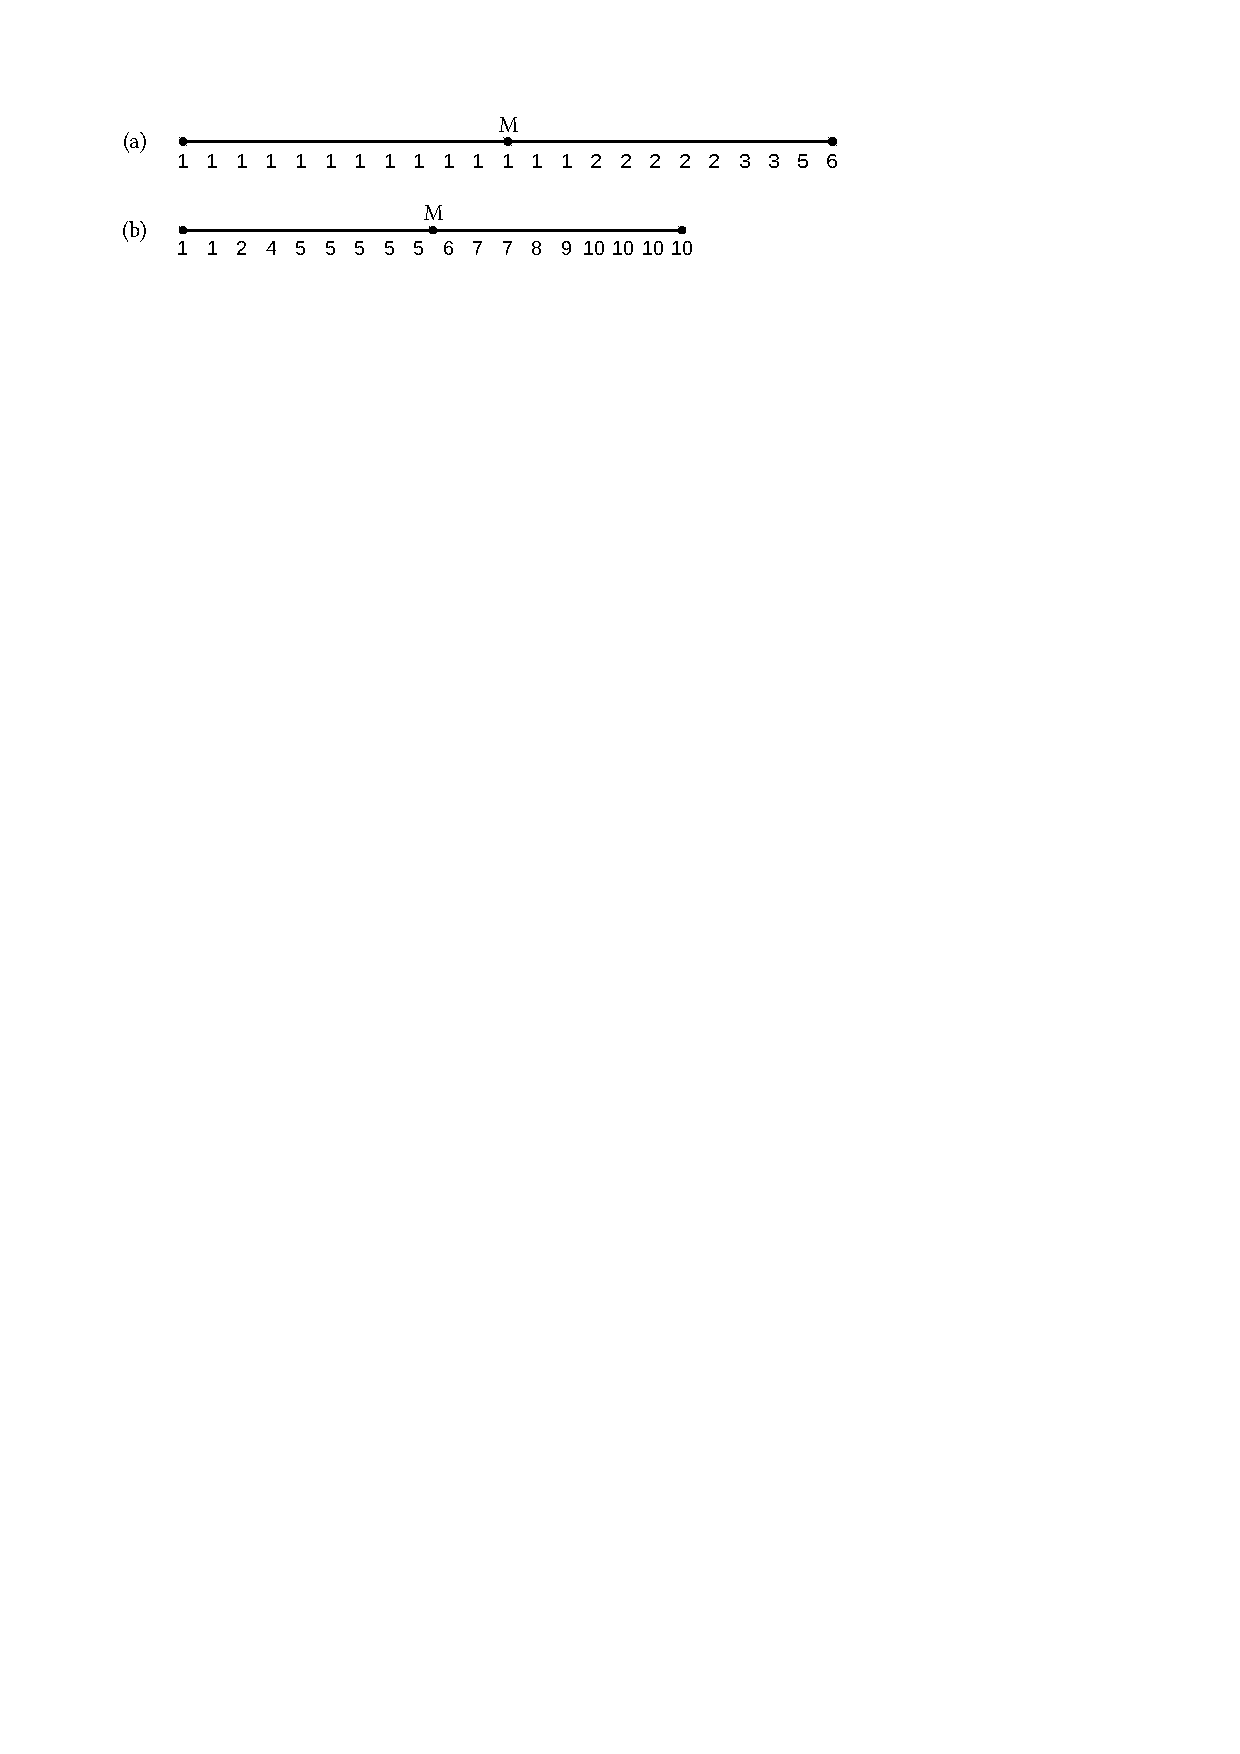
\includegraphics{figures/medians}
\end{figure}
% a)  1 1 1 1 1 1 1 1 1 1 1 \textbf{1} 1 1 2 2 2 2 2 3 3 5 6
% b) 1 1 2 4 5 5 5 5 \textbf{5 6} 7 7 8 9 10 10 10 10

If the sample consists of an even number of data points, we simply calculate the mean between the two values that lie in the middle of the ordered data set. For example, the rank values for the Animacy of our sample of \textit{of}-possessives are shown in Figure \ref{fig:possmedians}b. There are 18 values, so the median falls between the ninth and the tenth value (marked again by a dot labeled M). The ninth and tenth value are 5 and 6 respectively, so the median for the \textit{of}-possessive modifiers is $\nicefrac{(5+6)}{2} = 5.5$ (i.e., it falls between \textvv{concrete touchable} and \textvv{concrete nontouchable}).

Using the idea of a median, we can now rephrase our prediction in quantitative terms:

\begin{exe}
\ex \textit{Prediction}: The modifiers of the \textvv{\textit{s}-possessive} will have a higher median on the \textvv{Animacy} scale than the the modifiers of the \textvv{\textit{of}-possessive}.
\label{ex:animacypredictionrank}
\end{exe}

Our data conform to this prediction, as 1 is higher on the scale than 5.5. As before, this does not prove or disprove anything, as, again, we would expect some random variation. Again, we will return to this issue in Chapter \ref{ch:significancetesting}.

\subsection{Frequency lists and mode}
\label{sec:mode}

Recall that I mentioned above the possibility of treating ordinal data like nominal data. Table \ref{tab:relfreqpossmod} shows the relative frequencies for each animacy category, (alternatively, we could also calculate expected frequencies in the way described in Section \ref{sec:descriptiveordinal} above).

\begin{table}[!htbp]
\caption{Relative frequencies for the Animacy values of possessive modifiers}
\label{tab:relfreqpossmod}
\begin{tabular}[t]{rlcccc}
\lsptoprule
\multicolumn{2}{l}{\textvv{Animacy}} & \multicolumn{2}{c}{\textvv{\textit{s}-possessive}} &  \multicolumn{2}{c}{\textvv{\textit{of}-possessive}}  \\
Rank & Category & Abs. & Rel. & Abs. & Rel. \\
\midrule
1 & \textvv{human} & 14 & 0.609 & 2 & 0.111 \\
2 & \textvv{organization} & 5 & 0.217 & 1 & 0.056 \\
3 & \textvv{other animate} & 2 & 0.087 & 0 & -- \\
4 & \textvv{human attribute} & 0 & -- & 1 & 0.056 \\
5 & \textvv{concrete touchable} & 1 & 0.043 & 5 & 0.279 \\
6 & \textvv{concrete nontouchable} & 1 & 0.043 & 1 & 0.056 \\
7 & \textvv{location} & 0 & -- & 1 & 0.056 \\
8 & \textvv{time} & 0 & -- & 1 & 0.056 \\
9 & \textvv{event} & 0 & -- & 2 & 0.111 \\
10 & \textvv{abstract} & 0 & -- & 4 & 0.222 \\
\midrule
\multicolumn{2}{l}{Total} & 23 & 1.000 & 18 & 1.000 \\
\lspbottomrule
\end{tabular}
\end{table}

This table also nicely shows the preference of the \textit{s}-possessive for animate modifiers (human, organization, other animate) and the preference of the \textit{of}-possessive for the categories lower on the hierarchy. The table also shows, however, that the modifiers of the \textit{of}-possessive are much more evenly distributed across the entire Animacy scale than those of the \textit{s}-possessive.

For completeness' sake, let me point out that there is a third measure of central tendency, that is especially suited to nominal data (but can also be applied to ordinal and cardinal data): the \textit{mode}. The mode is simply the most frequent value in a sample, so the modifiers of the \textit{of}-possessive have a mode of 5 (or \textvv{concrete touchable}) and those of the \textit{s}-possessive has a mode of 1 (or \textvv{human}) with respect to animacy (similarly, we could have said that the mode of \textit{s}-possessive modifiers is \textvv{discourse-old} and the mode of \textit{of}-possessive modifiers is \textvv{discourse-new}. There may be more than one mode in a given sample. For example, if we had found just a single additional modifier of the type \textvv{abstract} in the sample above (which could easily have happened), its frequency would also be five; in this case, the \textit{of}-possessive modifier would have two modes (\textvv{concrete touchable} and \textvv{abstract}). 

The concept of \textit{mode} may seem useful in cases where we are looking for a single value by which to characterize a set of nominal data, but on closer inspection it turns out that it does not actually tell us very much: it tells us, what the most frequent value is, but not, how much more frequent that value is than the next most frequent one, how many other values occur in the data at all, etc. Thus, it is always preferable to report the frequencies of all values, and, in fact, I have never come across a corpus-linguistic study reporting modes.

\section{Descriptive statistics for cardinal data}
\label{sec:descriptivecardinal}

Let us turn, finally, to a design with one nominal and one cardinal variable: a test of the third of the three hypotheses introduced at the beginning of this chapter. Again, it is restated here together with the background assumption from which it is derived:

\begin{exe}
\ex Assumption: Short items tend to occur toward the beginning of a constiutent, long items tend to occur at the end. \\
Hypothesis: The \textvv{\textit{s}-possessive} will be used with short modifiers, the \textvv{\textit{of}-possessive} will be used with long modifiers.
\label{ex:lengthhypothesis}
\end{exe}

The constructions are operationalized as before. The data used are based on the same data set as before, except that cases with proper names and pronouns are excluded. The reason for this is that we already know from the first case study that pronouns, which we used as an operational definition of ``old information'' prefer the \textit{s}-possessive. Since all pronouns are very short (regardless of whether we measure their lenght in terms of words, syllables or letters), including them would bias our data in favor of the hypothesis. This left 20 cases of the \textit{s}-possessive and 154 cases of the \textit{of}-possessive. To get samples of roughly equal size for expository clarity, let us select every sixth case of the \textit{of}-possessive, giving us 25 cases (note that in a real study, there would be no good reason to create such roughly equal sample sizes -- we would simply use all the data we have).

The variable \textvv{Length} was defined operationally as ``number of orthographic words''. We can now state the following prediction:

\begin{exe}
\ex \textit{Prediction}: The mean length of modifiers of the \textvv{\textit{s}-possessive} should be smaller than that of the modifiers of the \textvv{\textit{of}-possessive}.
\label{ex:lengthprediction}
\end{exe}

Table \ref{tab:samplelengthsgenofc} shows the length of head and modifier for all cases in our sample.

\begin{table}[!htbp]
\caption{A sample of \textit{s}- and \textit{of}-possessives annotated for length of head and modifier (BROWN)}
\label{tab:samplelengthsgenofc}
\resizebox*{!}{\textheight}{
\begin{tabular}[t]{rlrr}
\lsptoprule
No. & Example & Modifier & Head \\
\midrule
(a) & \multicolumn{3}{l}{\textvv{\textit{s}-possessive}} \\
\midrule
1 & \makecell[lt]{\textit{the government's special ceremonies at Memorial University} \\ \textit{honoring distinguished sons and daughters of the island province}} & 2 & 14 \\
2 & \textit{the year's grist of nearly 15,000 book titles} & 2 & 6 \\
3 & \textit{a burgomaster's Beethoven} & 2 & 1 \\
4 & \textit{the world's finest fall coloring} & 2 & 3 \\
5 & \textit{a standard internist's text} & 3 & 1 \\
6 & \textit{mom's apple pie} & 1 & 2 \\
7 & \textit{the Square's historic value} & 2 & 2 \\
8 & \textit{his mother's urging} & 2 & 1 \\
9 & \textit{the Department's recommendation} & 2 & 1 \\
10 & \textit{the posse's apPROach} & 2 & 1 \\
11 & \textit{ladies' fashions} & 1 & 1 \\
12 & \textit{the convict's climactic reappearance in London} & 2 & 4 \\
13 & \textit{industry's main criticism of the Navy's antisubmarine effort} & 1 & 7 \\
14 & \textit{the town marshal's office} & 3 & 1 \\
15 & \textit{the pool's edge} & 2 & 1 \\
16 & \textit{man's tongue} & 1 & 1 \\
17 & \textit{an egotist's rage for fame} & 2 & 3 \\
18 & \textit{a women's floor} & 2 & 1 \\
19 & \textit{these shores' peculiar powers of stimulation} & 2 & 4 \\
20 & \textit{the novelist's carping phrase} & 2 & 2 \\
\midrule
(b) & \multicolumn{3}{l}{\textvv{\textit{of}-possessive}} \\
\midrule
 1  & \textit{the announcement last week of the forthcoming encounter} & 3 & 4 \\
 2  & \textit{the necessity of interpretation by a Biblical scholar} & 5 & 2 \\
 3  & \textit{his portrayal of an edgy head-in-the-clouds artist} & 4 & 2 \\
 4  & \textit{a lack of unity of purpose and respect for heroic leadership} & 8 & 2 \\
 5  & \textit{the death throes of men who were shot before the paredon} & 7 & 3 \\
 6  & \textit{lack of rainfall} & 1 & 1 \\
 7  & \makecell[lt]{\textit{the amazing variety and power of reactions, attitudes,} \\ \textit{and emotions precipitated by the nude form}} & 9 & 5 \\
 8  & \textit{the wet end of the cork} & 2 & 3 \\
 9  & \textit{the constitution of his home state of Massachusetts} & 5 & 2 \\
10  & \textit{the spirit of the mad genius from Baker Street} & 6 & 2 \\
11  & \textit{Ann's own description of the scene} & 2 & 3 \\
12  & \textit{considerable criticism of its length} & 2 & 2 \\
13  & \textit{the exaltations of combat} & 1 & 2 \\
14  & \textit{the existence of Prandtl numbers reaching values of more than unity} & 8 & 2 \\
15  & \textit{the outstanding standard bearer of Mr.  Brown's tradition for accuracy} & 5 & 4 \\
16  & \textit{the growth of senile individuals} & 2 & 2 \\
17  & \textit{the totality of singular lines} & 2 & 2 \\
18  & \makecell[lt]{\textit{a consequence of the severe condition of perceived threat that persists } \\ \textit{unabated for the anxious child in an ambiguous sort of school environment}} & 20 & 2 \\
19  & \textit{the lead of the Russians} & 2 & 2 \\
20  & \textit{costs of service} & 1 & 1 \\
21  & \textit{ineffective dispersion of stock ownership} & 2 & 2 \\
22  & \textit{the value of a for the major portion of the knife} & 8 & 2 \\
23  & \textit{the eyes of the Lord's servants} & 3 & 2 \\
24  & \textit{the high ridge of the mountains} & 2 & 3 \\
25  & \textit{the pirouette of his arms} & 2 & 2 \\
\lspbottomrule
\end{tabular}}
\end{table}
samplelengthsgenofc

\subsection{Means}
\label{sec:means}

How to calculate a mean (more precisely, an arithmetic mean) is common knowledge, but for completeness' sake, here is the formula:

\begin{exe}
\ex $\displaystyle{\overline{x}_{arithm} =  \frac{1}{n}\sum _{i=1}^nx_i = \frac{x_1+x_2+...+x_n}{n}}$ 
\label{ex:formulamean}
\end{exe}

In other words, in order to calculate the mean of a set of values $x_1, x_2, ..., x_n$ of size n, we add up all values and divide them by \textit{n} (or multiply them by $\nicefrac{1}{n}$, which is the same thing).

Since we have stated our hypothesis and the corresponding prediction only in terms of the modifier, we should first make sure that the heads of the two possessives do not differ greatly in length: if they did, any differences we find for the modifiers could simply be related to the fact that one of the constructions may be longer in general than the other. Adding up all 20 values for the \textit{s}-possessive heads gives us a total of 57, so the mean is $\nicefrac{57}{20} = 2.85$. Adding up all 25 values of the \textit{of}-possessive heads gives us a total of 59, so the mean is $\nicefrac{59}{25} = 2.36$. We have, as yet, no way of telling whether this difference could be due to chance, but the two values are so close together that we will assume so for now. In fact, note that there is one obvious outlier (a value that is much bigger than the others: Example (a 1) in Table \ref{tab:samplelengthsgenofc} has a head that is 14 words long. If we assume that this is somehow exceptional and remove this value, we get a mean length of $\nicefrac{43}{19} = 2.26$, which is almost identical to the mean length of the \textit{of}-possessive's modifiers.

If we apply the same formula to the modifiers, however, we find that they differ substantially: the mean length of the \textit{s}-possessive modifiers is $\nicefrac{38}{20} = 1.9$, while and the mean length of the \textit{of}-possessive's modifiers is more than twice as much, namely $\nicefrac{112}{25} = 4.48$. Even if we remove the obvious outlier, example (b 18) in Table \ref{tab:samplelengthsgenofc}, the \textit{of}-possessive's modifiers are twice as long as those of the \textit{s}-possessive, namely $\nicefrac{92}{24} = 3.83$.

\section{Summary}
\label{sec:datatypessummary}

We have looked at three case studies, one involving nominal, one ordinal and one cardinal data. In each case, we were able to state a hypothesis and derive a quantitative prediction from it. Using appropriate descriptive statistics (percentages, observed and expected frequencies, modes, medians and means), we were able to determine that the data conform to these predictions -- i.e., that the quantitative distribution of the values of the variables \textvv{Part of Speech}, \textvv{Animacy} and \textvv{Length} across the conditions \textvv{\textit{s}-possessive} and \textvv{\textit{of}-possessive} fits the predictions formulated.

However, these distributions by themselves do not prove (or, more precisely, \textit{fail to disprove}) the hypotheses for two related reasons. First, the predictions are stated in relative terms, i.e. in terms of more-or-less, but they do not tell us \textit{how much} more or less we should expect to observe. Second, we do not know, and currently have no way of determining, whether the more-or-less that we observe reflects real differences in distribution, or whether it falls within the range of random variation that we always expect when observing tendencies. More generally, we do not know how to apply the Popperian all-or-nothing research logic to quantitative predictions. All this will be the topic of the next chapter.
